Early neuroanatomists had different ideas of how the brain was composed, some stated that it was a continuous organ, that is neurons were fused into a single mesh of cells with no separation. In the early 1900, Ramón y Cajal demonstrated that nervous system consisted of individual cells and that they communicated through different parts of their anatomy~\cite{Nemri:2010}. Figure~\ref{fig:neuro:ramon-y-cajal-neuro} shows one of his many drawings, it portraits different neurons located near muscular tissue.

\begin{figure}[hbt]
  \begin{center}
    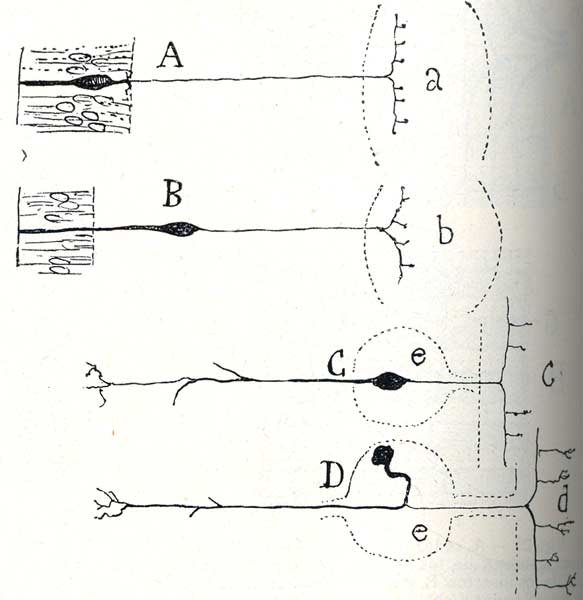
\includegraphics[width=0.45\textwidth]{ramon-y-cajal-fig_030}
    \caption{One of many Ramón y Cajal's drawings~\cite{cervantes-images}}
    \label{fig:neuro:ramon-y-cajal-neuro}
  \end{center}
\end{figure}

These cells are called \emph{neurons} and they are particularly good at  long-range communication~\cite{thompson2000brain}. While most cells in the body can ``talk'' to their neighbours, neurons have structures that allow them to communicate for up to a meter~\cite{eye-brain-vision-hubel1995}. The flow of information through the billions of neurons in the brain is what originates behaviour, this is an amazing fact that has led many scientists to focus their minds into this phenomenon.

\subsection{Basic neural structure}

Neurons are composed of a \emph{soma} or body, this part has similar components to other cells in the body; and specialized communication structures called the \emph{axon} and \emph{dendrites}. The \textbf{neuron soma} has many similar elements to other cells in the human body (e.g. nucleus, mitochondria, Golgi apparatus). All the neuron is enclosed in the cell membrane, just like any other cell. The soma is the biggest shape at the left of Figure~\ref{fig:neuro:neuron-anatomy}. \textbf{Dendrites} are ramifications that come off the soma and, in most cases, are used as receivers of information from other neurons (red branch-like structures at the left of Figure~\ref{fig:neuro:neuron-anatomy}). The shape of dendrites allows the nerve cell to have a larger contact area. For some neurons, dendritic branches have ``spines'', these are synapses formed with another neuron.

\begin{figure}
  \begin{center}
    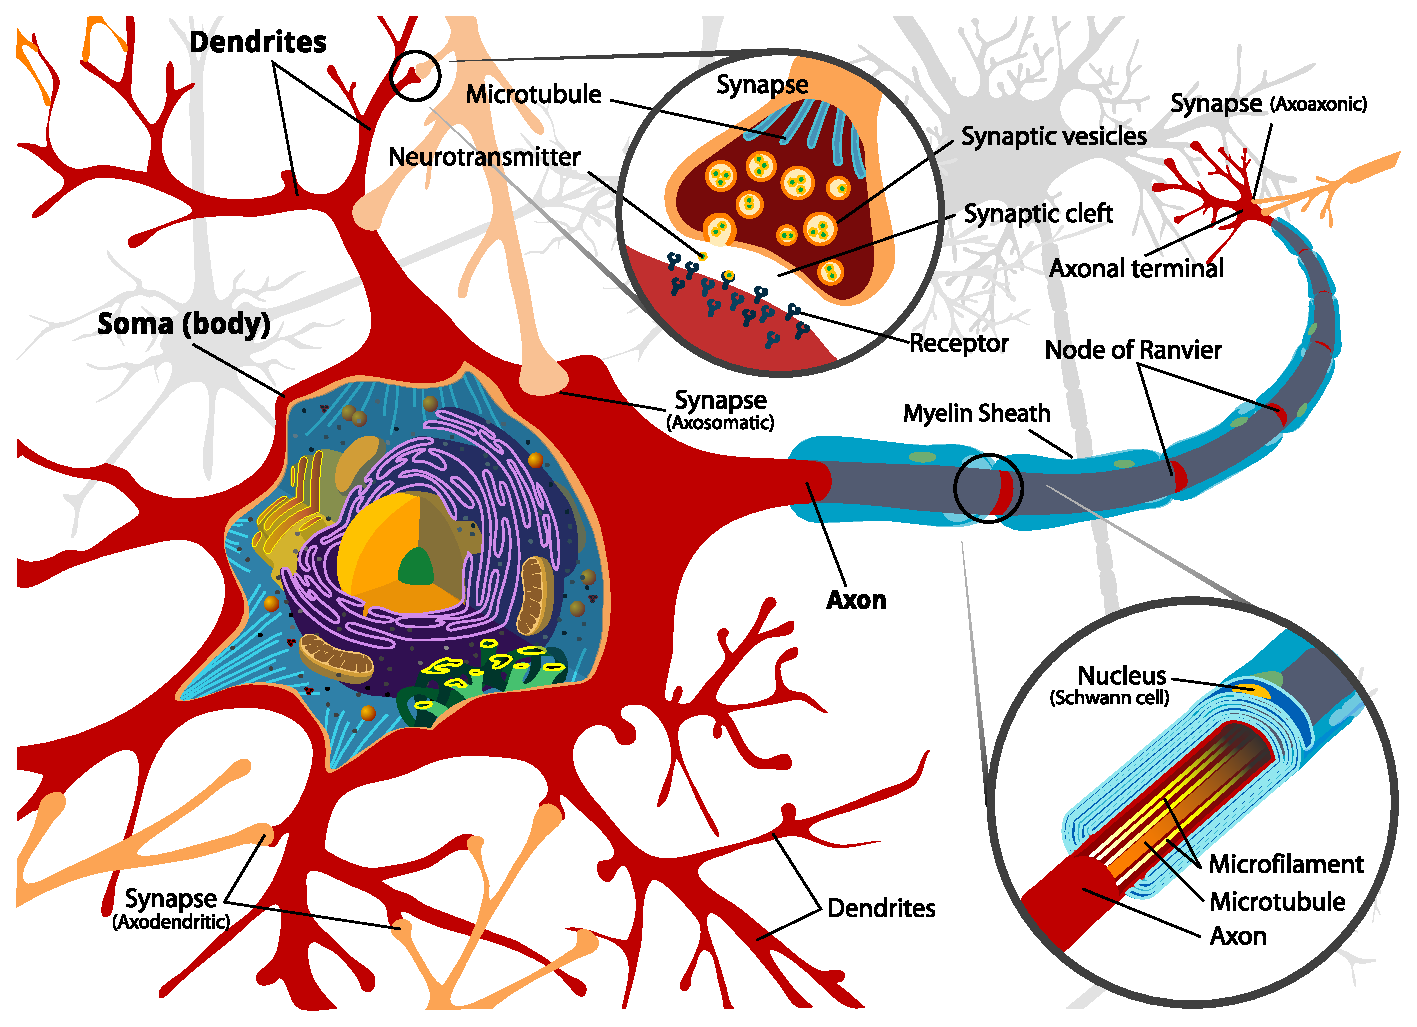
\includegraphics[width=\textwidth]{not-so-Complete_neuron_cell_diagram_en}
    \caption{Principal components of a neuron.}
    \label{fig:neuro:neuron-anatomy}
  \end{center}
\end{figure}

The other specialized communication element of nerve cells is the \textbf{axon}, it's at the other end of the information exchange and can be seen as an output of the neuron. It usually has elongated tubular shape and ramifications at its end, shown at the right of Figure~\ref{fig:neuro:neuron-anatomy}. As with dendrites, the tree-like shape at the end of the axon permits larger contact area, thus, more neurons can interconnect. The middle portion of the axon may, sometimes, be covered by a thin layer \emph{myelin}; a substance that acts as an insulator and improves signal transmission~\cite{thompson2000brain}. Although this is the basic way nerve cells communicate, there are variations that have been recently discovered and are subject of the late research efforts~\cite{Bullock04112005}.

The place where \textbf{synapse}
Theories suggest they perform some kind of calculation, most of the time modelled as a threshold activation function

Some neurons use analog/continuous signals to transmit information, though they are mostly act as an interface to the exterior world.

Latest evidence suggests that the complex cognitive functions are performed using spikes, on-off responses, as a means for communication.

The place where axons and dendrites meet, is called the SSS, synapses

When one neuron's output elicits another neuron to spike, 

\subsection{Neuron models}

From the very detailed Hudxley
Integrate and fire
Leaky integrate and fire
izhikevich simple model *choose this! :P